\section{Experimental Methods}

\subsection{\label{sec:setup} Experimental setup}

\begin{figure}[h]
    \centering
    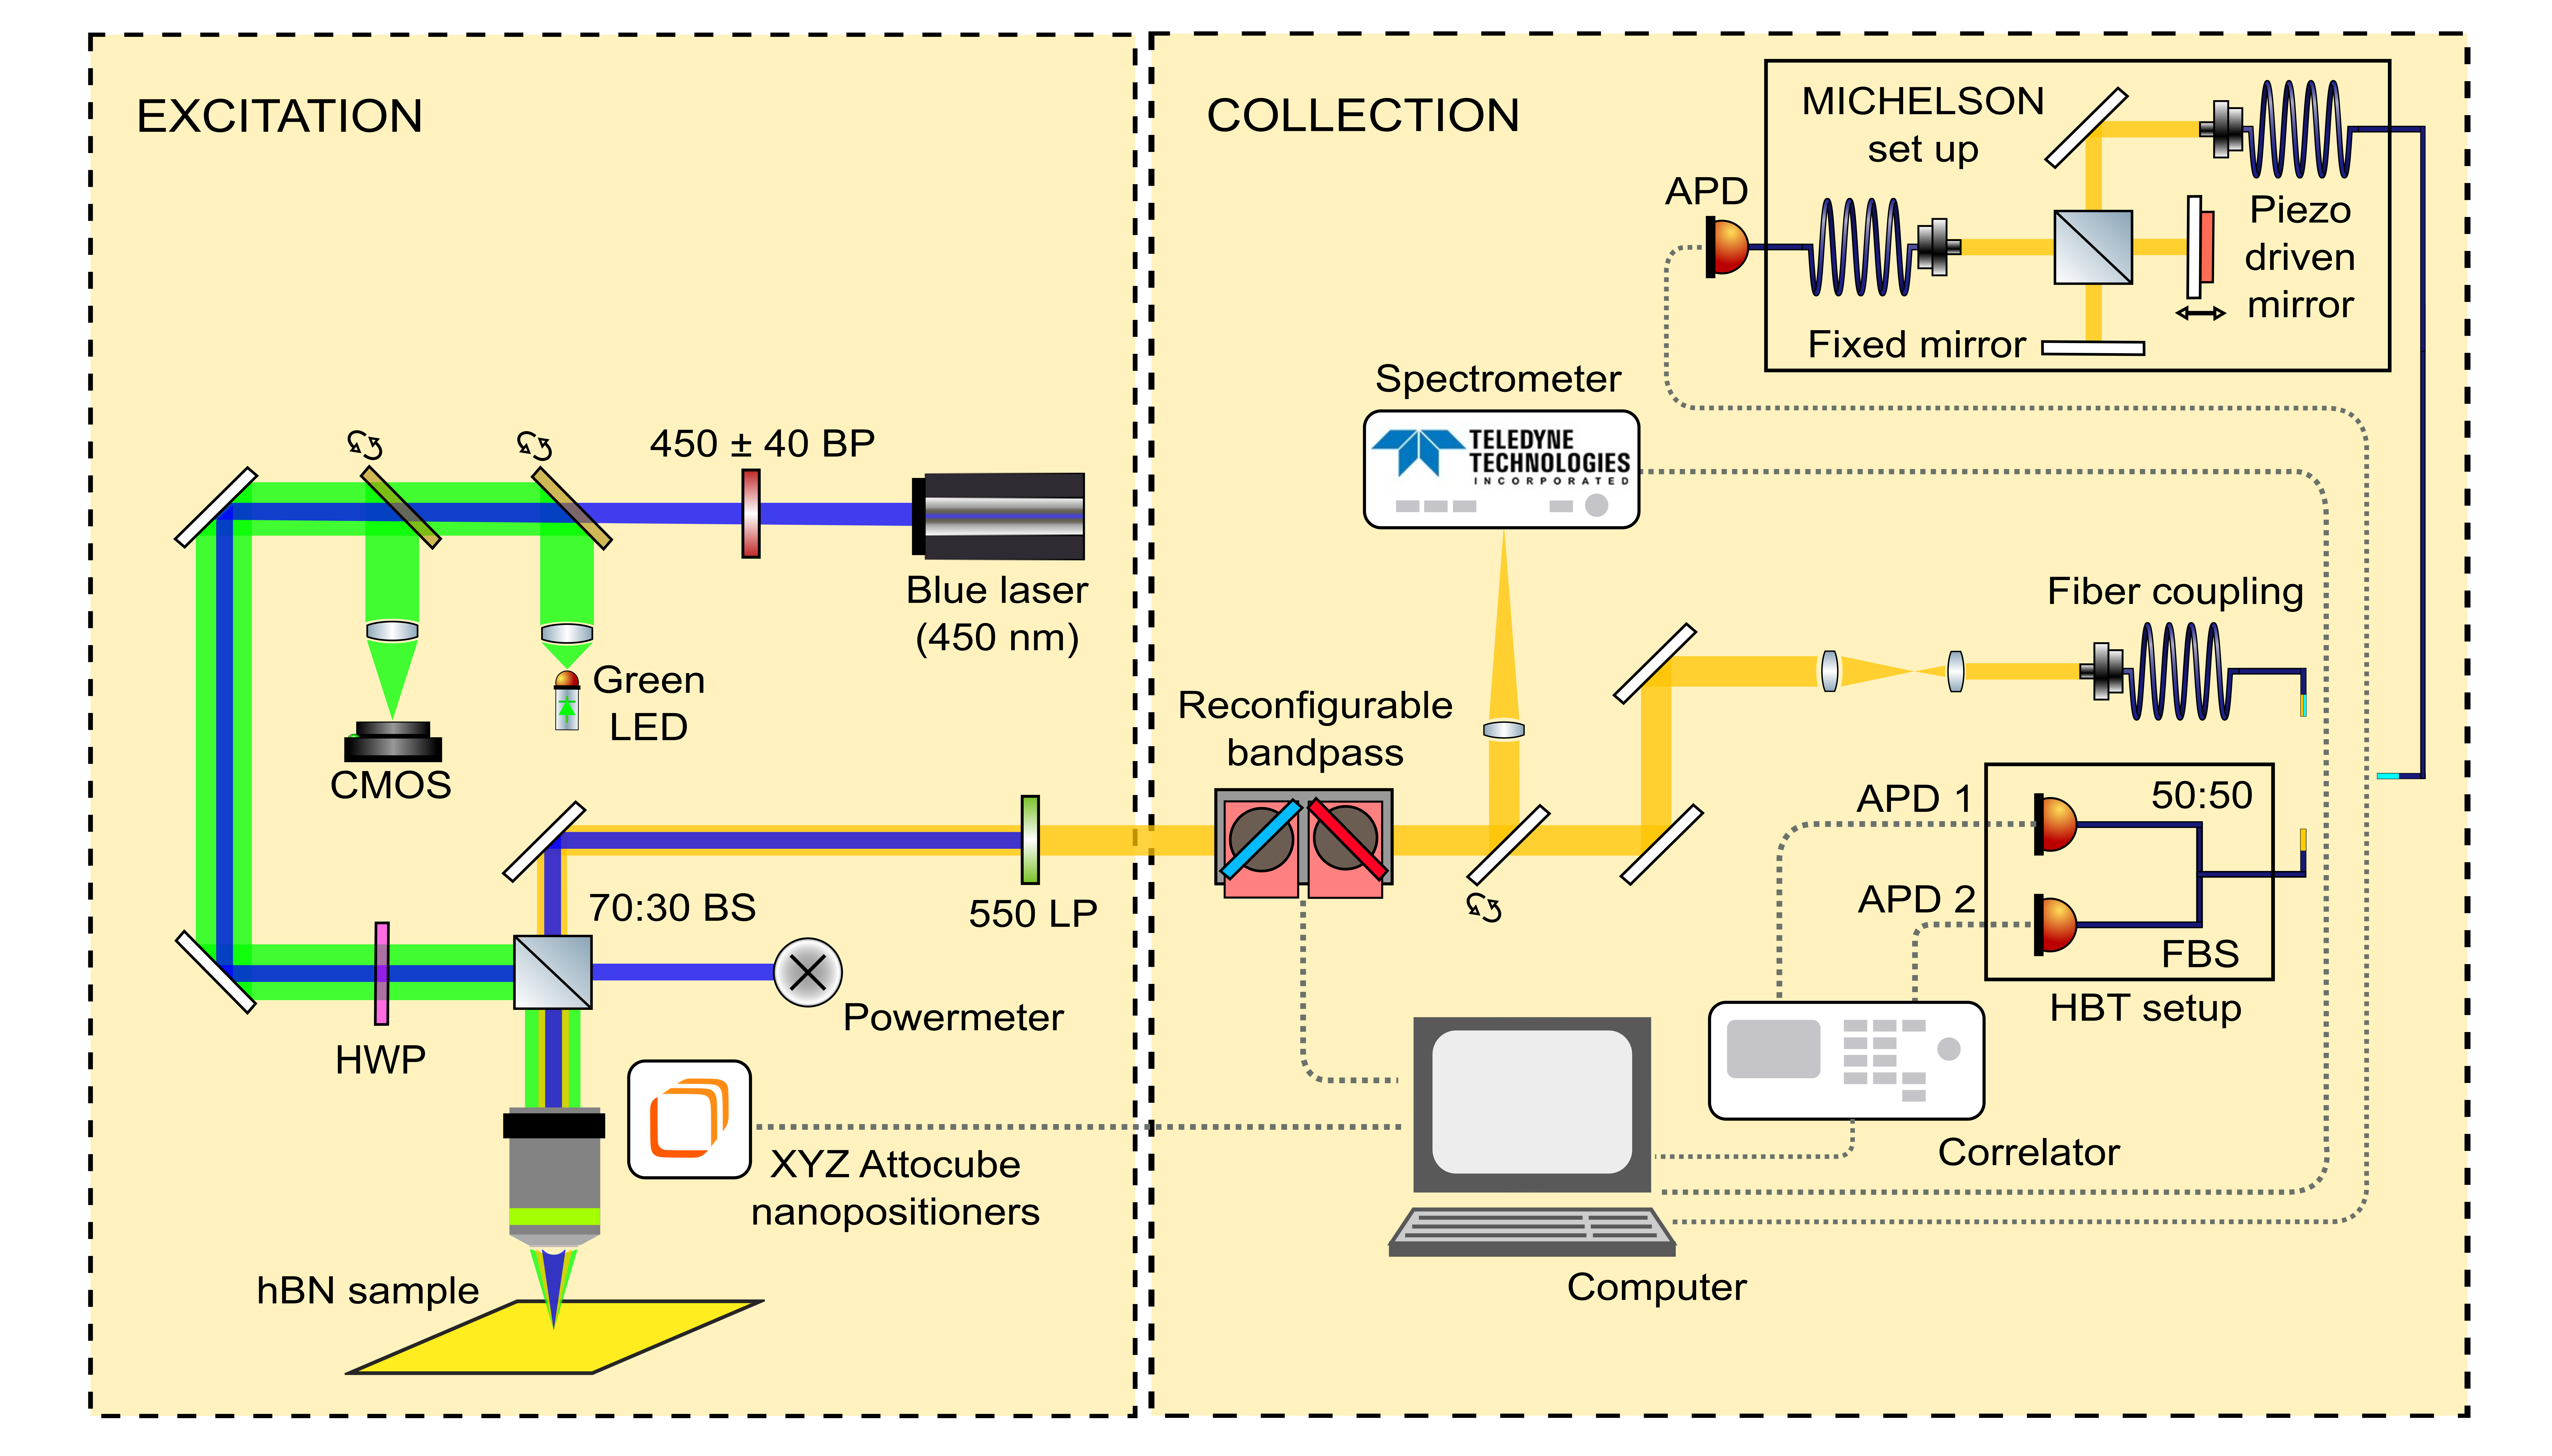
\includegraphics[width=1\linewidth]{Figures/ExperimentalSetUp.png}
    \caption{Graphic of the confocal microscopy setup used for the excitation and collection of emission from hBN defects. A 450~nm blue laser is used for excitation, while a green LED and a CMOS camera are used to visualise the sample on a computer screen. A 30:70 beam splitter reflects the excitation laser onto the sample and transmits the collected emission into the detection path. The sample position can be controlled with nanometre accuracy in all three spacial dimensions with Attocube nanopositioners. The excitation laser is filtered out using a 550 nm longpass filter. A reconfigurable bandpass filter tunable between 615--710 nm allows further filtering of the collected emission. The filtered emission can be directed either to a spectrometer or coupled into a single-mode fibre, which can send the signal to either a fibre HBT setup or a Michelson interferometer.}
    \label{fig:setup}
\end{figure}

A confocal microscopy setup is used at room temperature for the non-resonant excitation and collection of PL from defect centres in hBN, as shown in Fig.~\ref{fig:setup}. Excitation is done using a blue 450~nm laser spectrally cleansed with a 450~$\pm$~40~nm bandpass filter. The laser’s polarisation is controlled using a half-wave plate to maximise emission from the defects. A 70:30 (transmission:reflection) beam splitter directs the laser onto the sample and transmits part of the beam to a powermeter, although its actual ratio at 450~nm was measured as 83:17. A Mitutoyo objective lens with a numerical aperture of 0.55, mounted on a New Focus micropositioner, focuses the excitation onto the sample and collects emitted photons. The hBN sample is positioned on a set of closed-loop XYZ Attocube nanopositioners for nanometric control. Although a dichroic mirror would have improved collection efficiency, frequent excitatin wavelength changes during the project made its use impractical.

To remove the excitation laser in the collection path, a 550~nm longpass filter is placed after the beam splitter. Emission is passed to a reconfigurable bandpass filter formed by a pair of motorised Semrock filters (704~nm shortpass and longpass), allowing a tunable passband filter between 615~nm and 710~nm with a minimum FWHM of 2~nm. The filtered signal can then be directed either to a spectrometer for spectral analysis or coupled into single-mode fibre.

The single-mode fibre is routed either to a fibre based HBT setup or to a Michelson interferometer. The HBT consists of a 50:50 fibre beam splitter and two avalanche photodiodes (APDs), with detection events sent to a QuTag time-correlated single-photon counting (TCSPC) module for correlation analysis. The Michelson interferometer, operating in free space, uses a 50:50 beam splitter and two mirrors, one fixed and the other mounted on a piezo actuator for micrometre displacements. The piezo itself is mounted on a motorised translation stage for coarse millimetre adjustment. The interferometer output is coupled into single-mode fibre and sent to an APD connected to the QuTag module for intensity measurements.



\subsubsection{Detection Scheme}

A Princeton Instruments spectrometer and CCD are used for spectral characterisation of the emitters. The spectrometer offers grating options of 150, 300, and 600 gratings per millimetre (g/mm), with the 300 g/mm grating mainly used as it provides a balance between spectral resolution and bandwidth. Two MPD fibre-coupled APDs are available in the laboratory for measurements requiring high timing resolution, offering a timing jitter of 40~ps (FWHM), a detection efficiency of approximately 28\% at 670~nm, and a dead time of 77~ns. For experiments prioritising photon collection efficiency, such as second-order correlation measurements, Thorlabs SPDMH2F detectors were used, which provide a typical timing resolution of 1~ns, a quantum efficiency around 70\% at 670~nm, and a dead time of 45~ns.

To fully characterise the timing performance of each APD, their instrument response functions (IRFs) were measured. The IRF describes the temporal spread in the detector’s response to an ideally instantaneous photon arrival, defining the effective timing resolution of the system. This was carried out using a pulsed Tsunami laser at 750~nm with a pulse width of approximately 3~ps, much shorter than the expected timing resolution of the APDs. Each pulse was split by a 50:50 beam splitter, sending one path to a fast photodiode to provide a reference trigger and the other through a fibre attenuator to the APD under test.

The trigger voltage levels for the APDs and the photodiode were selected such that the threshold corresponded to the point of maximum gradient of the respective electrical signal. For reference, the photodiode trigger signal was set to -116~mV. Table~\ref{tab:apd_characterisatoin} summarises the trigger voltages for each APD tested in the laboratory.


\begin{table}[h!]
\centering
\begin{tabular}{|c|c|}
\hline
\textbf{APD Label} & \textbf{Trigger voltage (V)}  \\
\hline
ThorLabs APD1 &     1.5            \\
\hline
Thorlabs APD2 &      1.2         \\
\hline
Thorlabs APD3 &      1.4       \\
\hline
Thorlabs APD4 &      1.3         \\
\hline
MPD APD1 &     1.5               \\
\hline
MPD APD2 &     1.5             \\
\hline
\end{tabular}
\caption{Trigger voltage for each APD}
\label{tab:apd_characterisatoin}
\end{table}

With the trigger level correctly set for each APD, second-order correlation data was collected between the reference signal from the photodiode and the subsequent detection signal from each APD, with a bin width of 1 ps. The results for Thorlabs APD1 and MPD APD1 are shown in Fig.~\ref{fig:apd-characterisation}. The FWHM of each APDs IRF was estimated in python by smoothing the raw data and measuring the FWHM of the smoothed curve. The APDs with the narrowest IRFs were selected for subsequent experiments to minimise timing uncertainty. MPD APD1 was used for lifetime measurements, while Thorlabs APD1 and APD3 were used for all other measurements.


\begin{figure}[h]
    \centering
    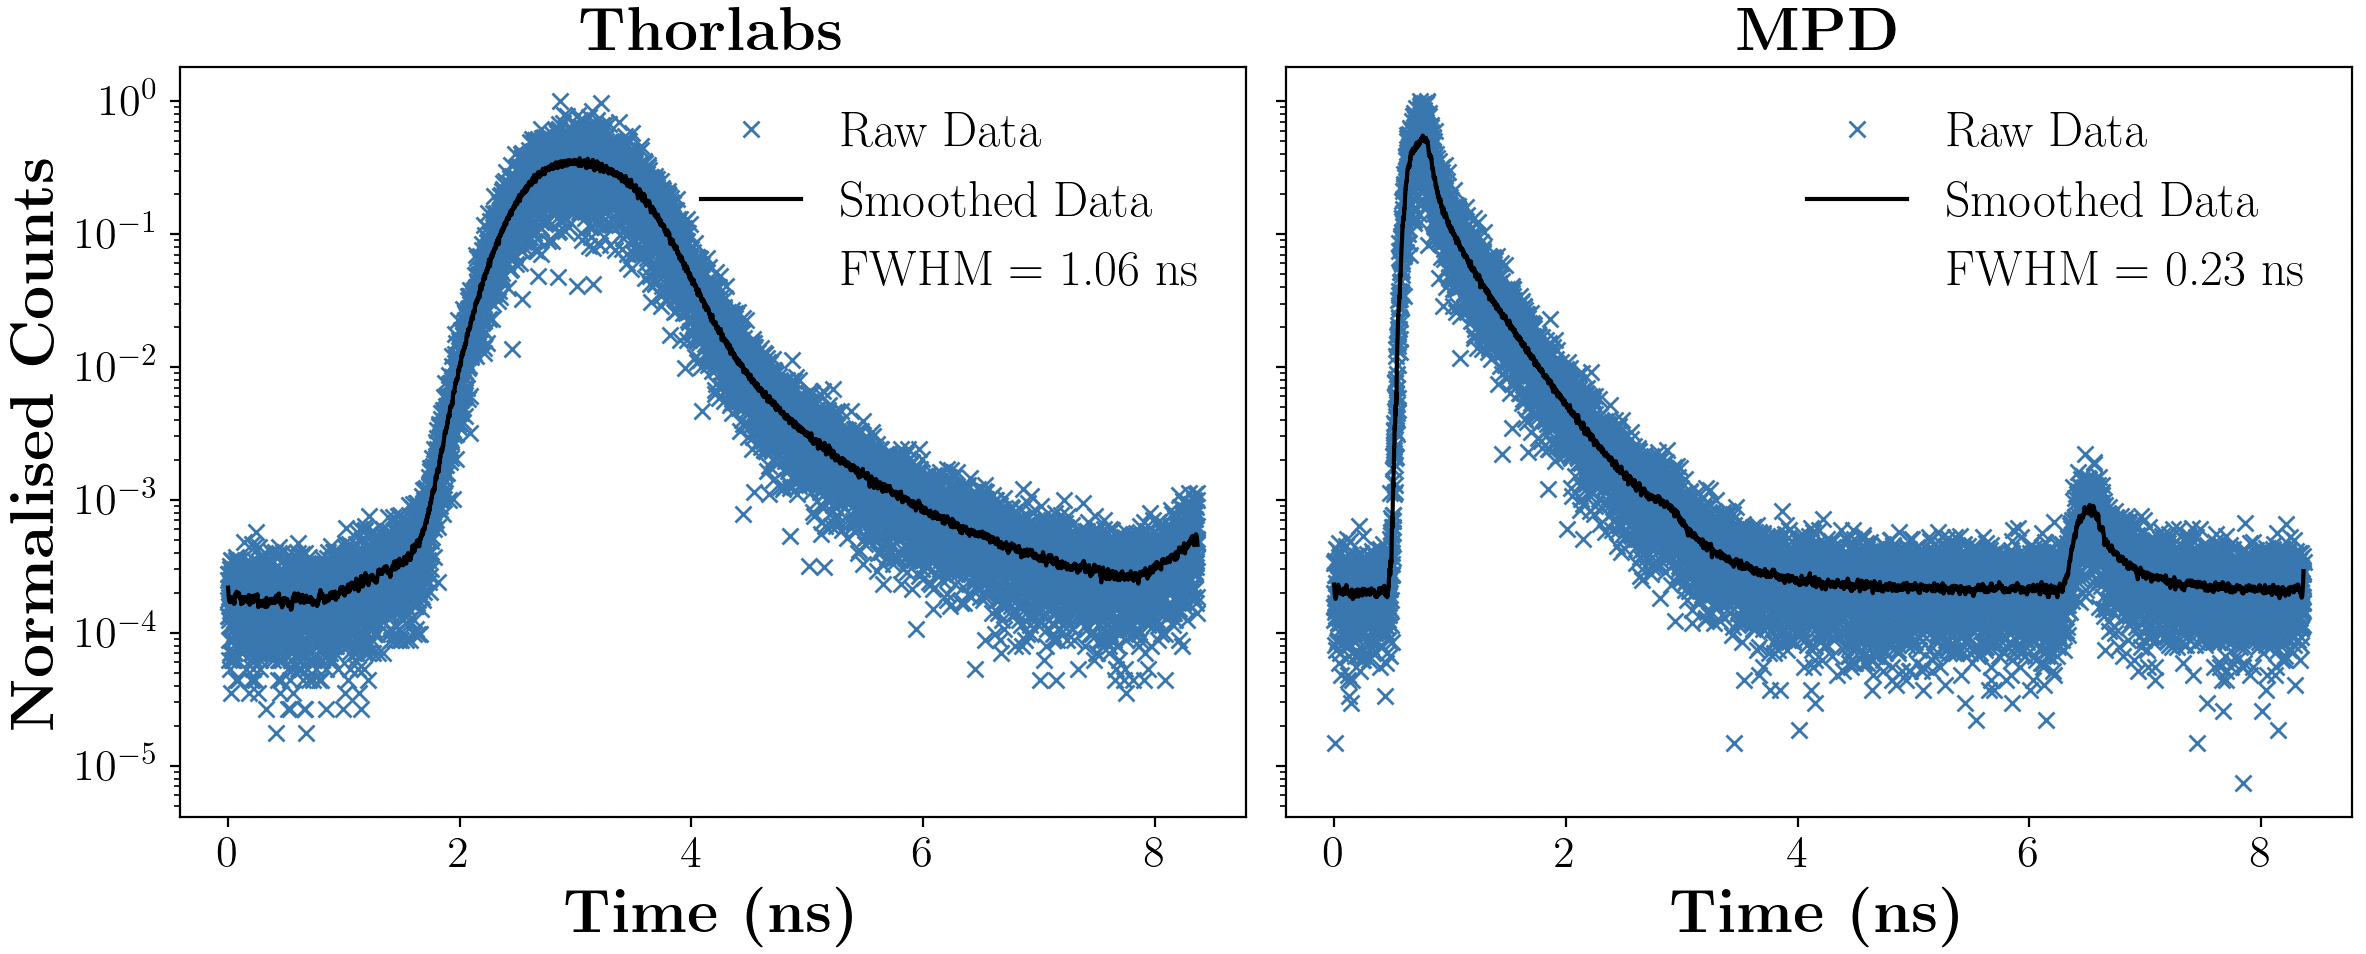
\includegraphics[width=0.9\linewidth]{Figures/APDChar.png}
    \caption{IRFs of two APDs measured using a 750~nm, $\sim$3~ps pulsed laser source. Raw data (green crosses) were smoothed using a Savitzky–Golay filter to extract the FWHM of the IRF (black line). The Thorlabs detector (a) exhibits an IRF of 1.06~ns FWHM, while the MPD detector (b) demonstrates significantly sharper timing with a 0.23~ns FWHM.}
    \label{fig:apd-characterisation}
\end{figure}

The IRFs of both APDs, shown in Fig.~\ref{fig:apd-characterisation}, reflect the inherent differences in their timing performance. The Thorlabs APD displays a broader, more symmetric IRF consistent with a Gaussian profile, indicating greater timing jitter and a slower response. In contrast, the MPD APD exhibits a much sharper, asymmetric IRF with a rapid rise and an extended tail, characteristic of fast triggering and high temporal resolution, but with potential contributions from afterpulsing or depletion from carriers in the APD \cite{Ziarkash2018}. The secondary peak observed at approximately 6.5~ns in the MPD APD trace, as well as the rising signal at the end of the Thorlabs APD trace, can also be attributed to afterpulsing effects.


\subsubsection{Laser Characterisation}

The laser employed was the PicoQuant LDH-IB-450-B laser head, controlled via a Taiko PDL M1 controller. It can operate in both CW and pulsed modes, and has a centre wavelength of 459~nm, as shown in Fig.~\ref{fig:laser-char}a.

\begin{figure}[h]
    \centering
    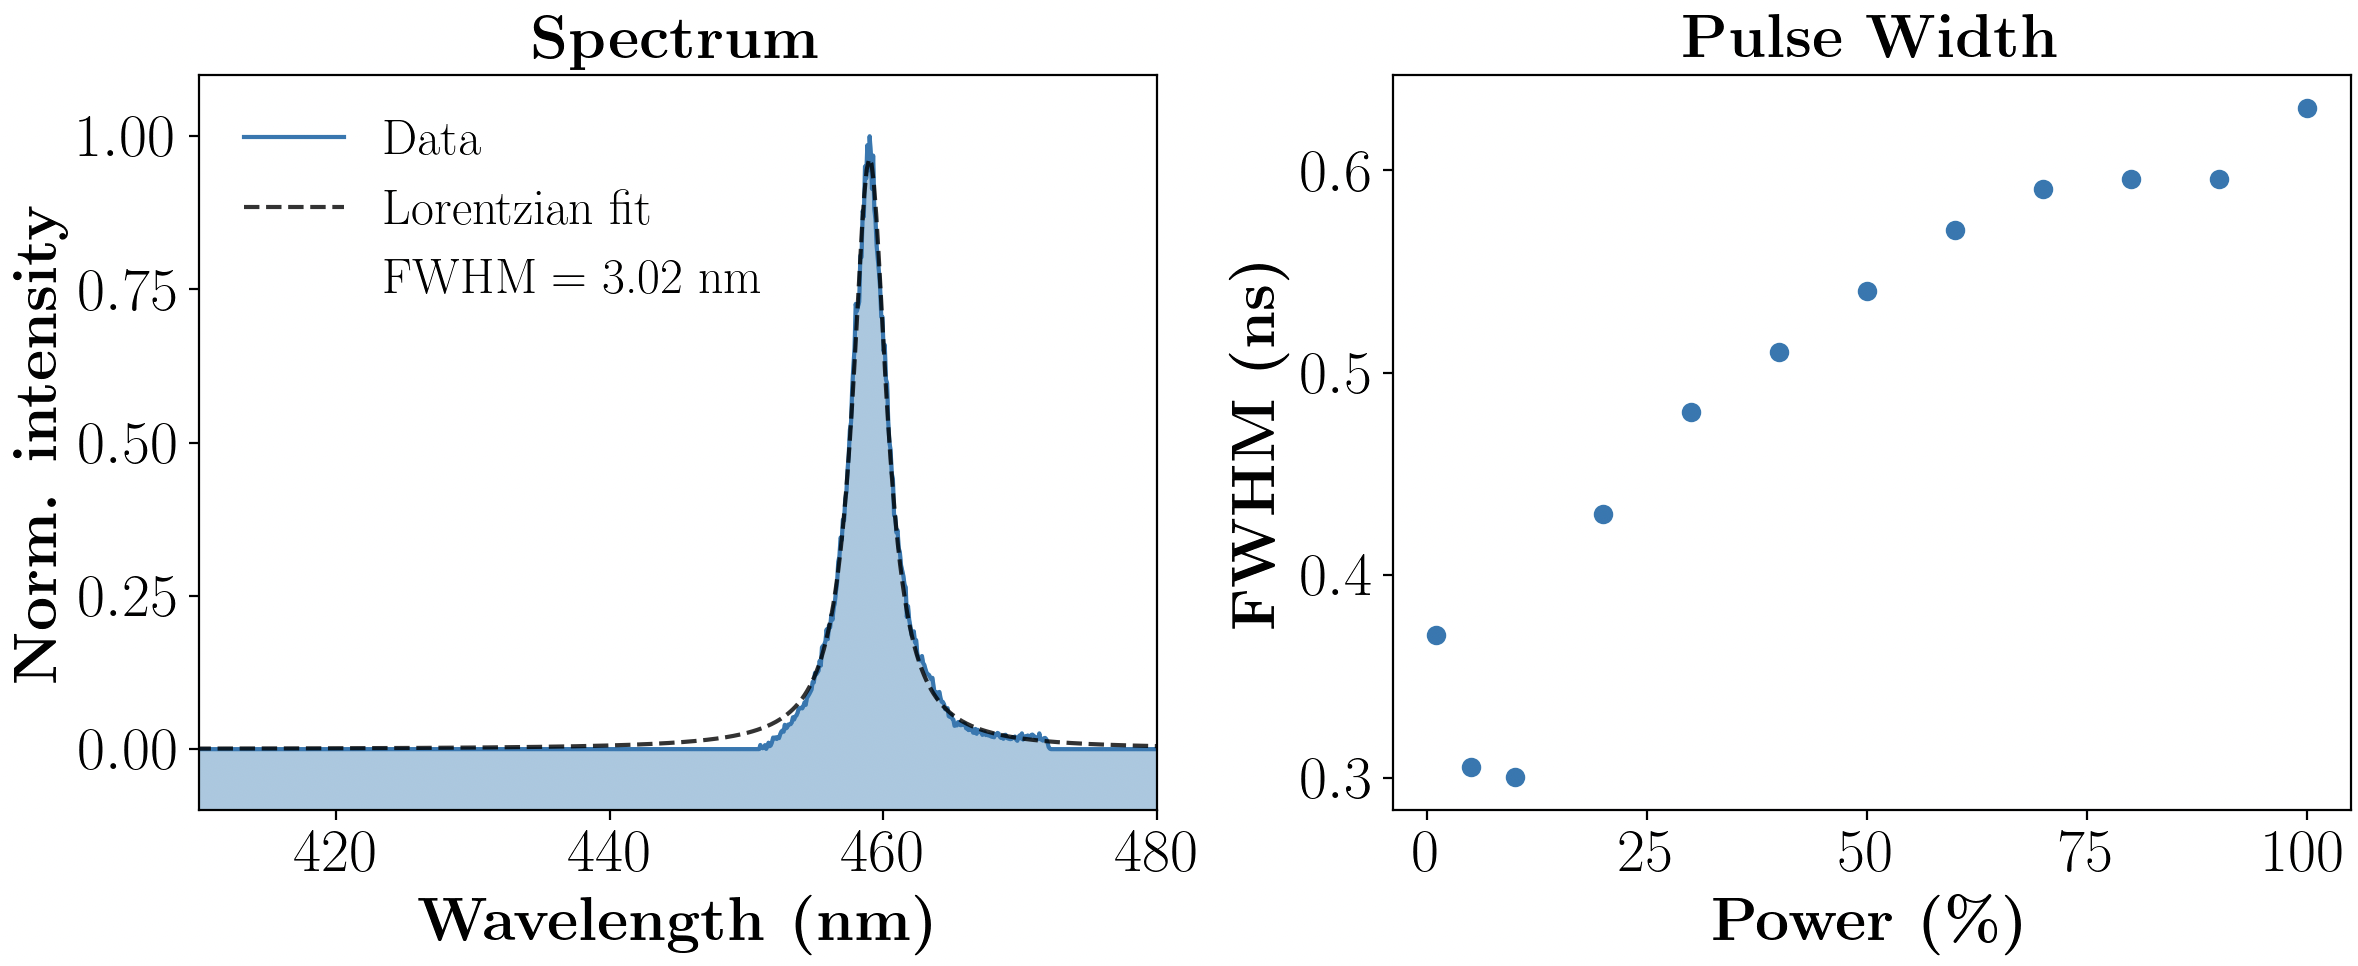
\includegraphics[width=1\linewidth]{Figures/LaserCharacterisation.png}
    \caption{Characterisation of the PicoQuant LDH-IB-450-B laser. (a) Emission spectrum fitted with a Lorentzian function to extract the centre wavelength and FWHM, which was found to be 3.02~nm. (b) Temporal shape of the pulse width at 10\% of the maximum laser power (c) Measured pulse width (FWHM) as a function of excitation power. A minimum pulse width is observed near 10\% laser power.}
    \label{fig:laser-char}
\end{figure}

The resulting spectrum was fitted with a Lorentzian function, yielding a FWHM of 3.02~nm. The use of the bandpass filter was essential to suppress background noise, particularly in the 550--650~nm range, not shown.

The pulse width of the emission was measured as a function of laser power using MPD APD1, Fig.~\ref{fig:laser-char}b,c. Although the measured FWHM values are close to the detector’s timing resolution and should ideally be deconvoluted from the IRF, the absolute values are not important, rather that they be minimised. This minimum pulse width occurs near 10\% excitation power Fig.~\ref{fig:laser-char}c, corresponding to approximately 0.048~mW on the source at a 40~MHz repetition rate.

Although the laser operates in free space, an attempt was made to couple it into a single-mode fibre using a fibre collimator. However, due to the high ellipticity of the beam, even with cylindrical lenses to correct the asymmetry, a maximum coupling efficiency of only $\sim$30\% was achieved. Nonetheless, coupling into single-mode fibres is generally desired, as it filters the spatial mode into a well-defined Gaussian profile. To investigate this further, a program was developed to optimise coupling efficiency. Maximising single-mode coupling requires precise mode-matching between the free-space beam and the fibre output mode (the shape of the beam if it were emerging from the collimator). This is typically achieved using a telescope formed by two lenses of specific focal lengths. This condition can be verified experimentally by measuring the beam radius $w(z)$ as a function of propagation distance $z$ from both the laser head and the backwards-emitted collimated beam \cite{BahaaE.A.Saleh1991}.

To automate this process, a Python program was developed to determine the lens foci and spacing that best replicates the fibre-collimated beam profile. The program is based on Gaussian beam optics, where the beam radius as a function of propagation distance $z$ is described by:

\begin{equation}
    w(z) = w_0 \sqrt{1 + \left( \frac{z}{z_R} \right)^2},
    \label{eqn:beam-radius}
\end{equation}

where $w_0$ is the beam waist, and $z_R = \pi w_0^2 n / \lambda$ is the Rayleigh range, with $\lambda$ being the wavelength of the light and $n$ the refractive index of the medium. The beam radius $w(z)$ is defined as the radial distance at which the intensity drops to $1/e^2$ of its peak value.

The propagation of the Gaussian beam through optical elements is described using ABCD matrix formalism \cite{Popescu2022}. For free-space propagation over a distance $x$, and transmission through a thin lens of focal length $f$, the respective matrices are:

\begin{equation}
    T_{fs} =
    \begin{pmatrix}
        1 & x \\
        0 & 1 
    \end{pmatrix}, \quad
    T_{l} =
    \begin{pmatrix}
        1 & 0 \\
        -\frac{1}{f} & 1 
    \end{pmatrix}.
    \label{eqn:beam-tm}
\end{equation}

By multiplying the appropriate sequence of matrices, the evolution of the beam through a two-lens system can be computed to predict the beam profile at the fibre input. The program first fits the measured beam profiles from the laser and the fibre collimator to equation~\ref{eqn:beam-radius}, extracting the beam waist $w_0$ and Rayleigh range $z_R$. It then performs a numerical optimisation, using \texttt{scipy.optimize.minimize}, to minimise the mean squared error (MSE) between the calculated post-lens beam and the measured fibre-collimated profile. Constraints include a minimum distance between the laser and the first lens (to account for fixed optics) and the known distance to the fibre collimator. To avoid local minima, the optimisation runs 100 times with random initial parameters, retaining the configuration with the lowest MSE. The script evaluates all valid lens combinations specified by the user, returning the lens pair and positions yielding the closest match to the target beam, thereby maximising coupling efficiency. An example optimisation result is shown in Fig.~\ref{fig:optimised-telescope}, where the MSE was reduced to $9.3\times10^{-24}$ m$^2$, with the blue line showing the incoming beam and the red dashed line the ideal coupling profile.


\begin{figure}[h]
    \centering
    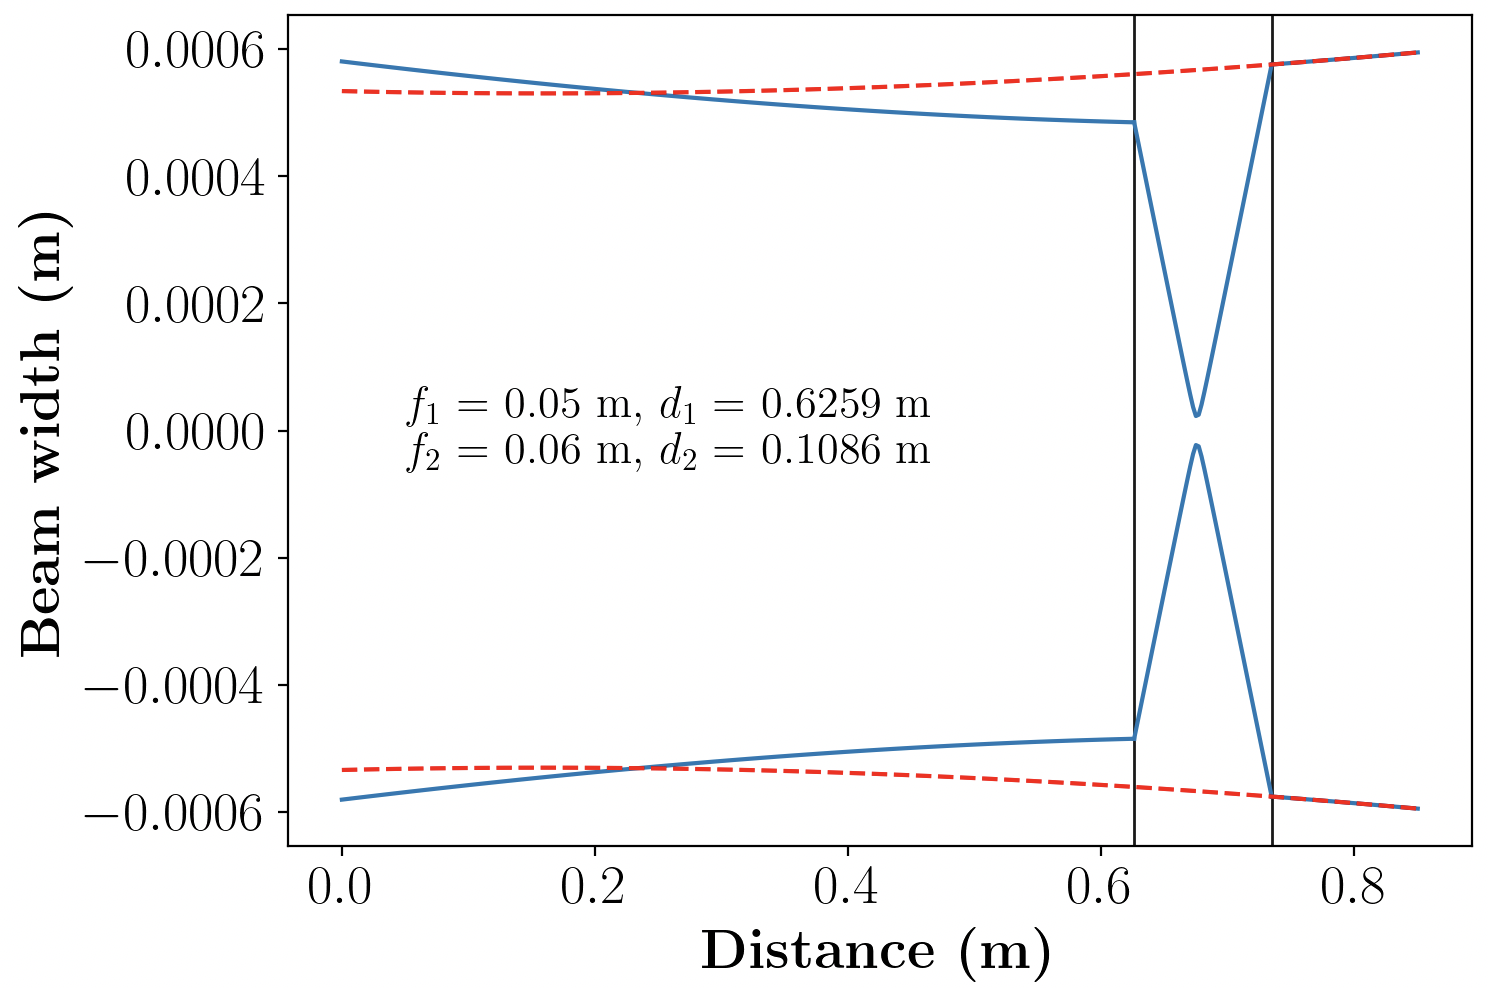
\includegraphics[width=0.9\linewidth]{Figures/OptimalTelescope.png}
    \caption{Beam propagation through the optimised telescope configuration for a laser used in a Mach–Zehnder interferometer in a separate setup. The blue curve shows the calculated Gaussian beam profile after passing through the selected lens pair, while the red dashed curve represents the target fibre-collimated beam profile. The lenses have focal lengths $f_1 = 0.05$~m and $f_2 = 0.06$~m, placed at distances $d_1 = 0.6259$~m and $d_2 = 0.1086+d_1$~m from the laser head respectively.}
    \label{fig:optimised-telescope}
\end{figure}


\subsection{Imaging Techniques}

Throughout this project, various search methods were employed to identify high-quality hBN defects. A suitable defect was defined as one that was spatially isolated from other emitters, exhibited a high signal-to-noise ratio, and demonstrated temporal stability under CW non-resonant excitation.

\subsubsection{APD Scanning Method and Wide Spot Excitation, \label{APD-scan}}

The first method used to search for emitters involved scanning a 10~$\mu$m~$\times$~10~$\mu$m area of the sample in a square grid, with the APD collecting counts at 250~nm step intervals. At each point, photon counts were recorded over a 100~ms integration time. This produced a spatial PL map of the region, from which individual emitters could be readily identified, as shown in Fig.~\ref{fig:search-tech}.

\begin{figure}
    \centering
    \includegraphics[width=0.9\linewidth]{Figures/SearchTech.png}
    \caption{a) Spatial PL map of a 10~$\mu$m~$\times$~10~$\mu$m region acquired via APD scanning. The scan was performed in 250~nm steps with 100~ms integration time at each position. Brighter regions correspond to higher photon counts, indicating potential emitter locations. b) Wide-spot excitation method for rapid emitter identification. A lens before the objective broadens the excitation beam on the sample, enabling larger-area illumination. Emission is directed to the spectrometer, where bright regions are quickly located by visualising the full sensor output in LightField.}
    \label{fig:search-tech}
\end{figure}

While effective at locating individual defects, this method is relatively inefficient due to the long acquisition time, approximately three minutes per scan, and the limited area covered, making it impractical for scanning large regions of the sample. An alternative approach was wide-spot imaging, achieved by placing a 20~mm focal length lens before the 70:30 beam splitter, Fig.~\ref{fig:setup}, to focus the excitation laser on the back focal plane of the objective. This produced a much larger spot on the sample surface, enabling excitation over a broad area. Emission was collected and directed to the spectrometer, with the full CCD sensor visualised in LightField software, allowing bright emitters to be identified instantly, considerably faster than the APD method.

While both the wide-spot and APD scanning techniques were effective at locating bright emitters, brightness alone did not guarantee high quality single-photon sources. In practice, many initially promising sites exhibited noisy or spectrally impure signals when examined, rendering them unsuitable for further study.

\subsubsection{Random Search and Spatial Referencing System}

The most efficient search method for locating bright, isolated defects was found to be a random search approach. In this method, a randomly chosen hBN flake, identified on the CMOS camera, was excited using the 450~nm laser, and the emission was directed to the spectrometer for real-time spectrum visualisation. A manual random walk was then performed using the Attocube nanopositioners, whereby the sample position was adjusted until either a suitable emitter was found or the search was abandoned and a new flake was selected. An example of hBN flakes visible on the CMOS during this process is shown in Fig.~\ref{fig:map}a.

\begin{figure}[h]
    \centering
    \includegraphics[width=0.9\linewidth]{Figures/Map.png}
    \caption{a) CMOS image showing multiple hBN flakes used in the random search method for identifying optically active defects. b) Full defect map of hBN sample}
    \label{fig:map}
\end{figure}


This method proved to be the most efficient and reliable for locating promising single-photon emitters. To ensure that identified emitters could be reliably revisited, a spatial referencing system was developed, and a map of each sample was created using a standard microscope to reconstruct the topography of the whole dropcast area, Fig.~\ref{fig:map}b. Two well-defined points on the hBN flake were selected to form a reference basis, and their coordinates were recorded using the closed-loop Attocube nanopositioners. Since the sample position could shift due to removal or mechanical drift, the reference points were re-measured at the start of each session. When a new emitter was found, its coordinates were transformed into the original reference frame using a custom program. An application built using \texttt{tkinter} was developed to automate this process and store all recorded emitter positions in a database, Fig.~\ref{fig:database}.

\begin{figure}
    \centering
    \includegraphics[width=0.9\linewidth]{Figures/database.png}
    \caption{Example of database created to track position of hBN defect emission. The left image shows part of the map sample, Fig.~\ref{fig:map}b, with emitters labelled. The right image is a snapshot of one of the databases used to keep track of the defect locations with respect to an origin.}
    \label{fig:database}
\end{figure}


\subsection{hBN Measurements}

\subsubsection{Lifetime and Saturation Curve}

Once an emitter with a suitable spectrum is identified, the first measurements performed are a saturation curve and lifetime. A saturation curve characterises how emission intensity varies with excitation power and can be measured under pulsed or CW excitation. The measurement is carried out using an isolated ZPL (using the tuneable bandpass), with the collection path directed to the HBT setup. In this context, the HBT setup is used purely for convenience: by summing photon counts from both APDs instead of analysing temporal correlations, it functions as a direct brightness measurement tool. A custom program automates the process by increasing excitation power in 5\% steps from 0\% to 100\%. At each step, the power is recorded with a powermeter and the total photon counts are integrated over 100~ms. The powermeter reading is converted to source power by multiplying by 17/83, the measured reflection:transmission ratio of the beam splitter at 450~nm. This process is repeated five times per power level, with the mean and standard deviation used to define the value and uncertainty of the intensity $I(P)$ at each excitation power $P$.


The resulting data is fitted with the standard saturation dependence of a two-level system under incoherent excitation:

\begin{equation}
    I(P) = \frac{P I_{\infty}}{P + P_{\text{sat}}},
    \label{eqn:p-sat}
\end{equation}

where $I_{\infty}$ is the theoretical maximum emission intensity at infinite excitation power, and $P_{\text{sat}}$ is the saturation power, defined as the excitation power at which the emitter reaches half of its maximum intensity. The brightness of an emitter measured at the detector, $B_d$, is estimated under CW excitation as $I_{\infty}\times T_1$, where it is limited by the decay rate $\gamma/2\pi=1/T_1$. Under pulsed excitation, brightness is given by $I_{\infty}\times R$, with $R$ being the laser repetition rate, which then sets the maximum brightness.

Emitter lifetimes are measured using pulsed excitation at 40~MHz repetition rate, with triger signals from the laser controller and detection signal from MPD APD1 fed into the QuTag TCSPC module. Data acquisition is performed with \textit{Daisy} \cite{zotero-item-9595}. Lifetime measurements help identify true single-photon sources: an ideal two-level system exhibits a single exponential decay, while multi-exponential decays indicate additional energy levels or overlapping defects. If the measured decay is consistent with a two-level system, the data is fitted with a single-exponential function:

\begin{equation}
    I(t) = A e^{-\gamma t},
    \label{eqn:lifetime}
\end{equation}

where $I(t)$ is the photon count rate at time $t$ after the trigger signal, $A$ is the initial amplitude (the maximum number of detected photons), and $\gamma$ is the spontaneous decay rate.


\subsubsection[Hanbury-Brown and Twiss]{Hanbury Brown and Twiss and $\mathbf{g^{(2)}(0)}$} \label{sec:g2}


The HBT setup, Fig.~\ref{fig:setup}, measures the second-order correlation function, $g^{(2)}(\tau)$, by recording the arrival times of photons detected by each APD. Data acquisition is carried out using the \textit{Tarec} (quTag Record \& Merge Tool) software, which logs a timestamp for every detection event. 

The HBT can be operated under both CW and pulsed excitation schemes. Under CW excitation, the correlation histogram is typically fitted using either a single- or bi-exponential decay function, depending on the underlying emitter dynamics. The single-exponential form is given by:

\begin{equation}
    g^{(2)}(\tau) = A + B e^{-\left| \gamma_1\tau \right|},
    \label{eqn:single-decay-g2}
\end{equation}

and the bi-exponential form is:

\begin{equation}
    g^{(2)}(\tau) = A + B e^{-\left| \gamma_1\tau \right|} + C e^{-\left| \gamma_2\tau \right|},
    \label{eqn:bi-decay-g2}
\end{equation}

\begin{figure}[h]
    \centering
    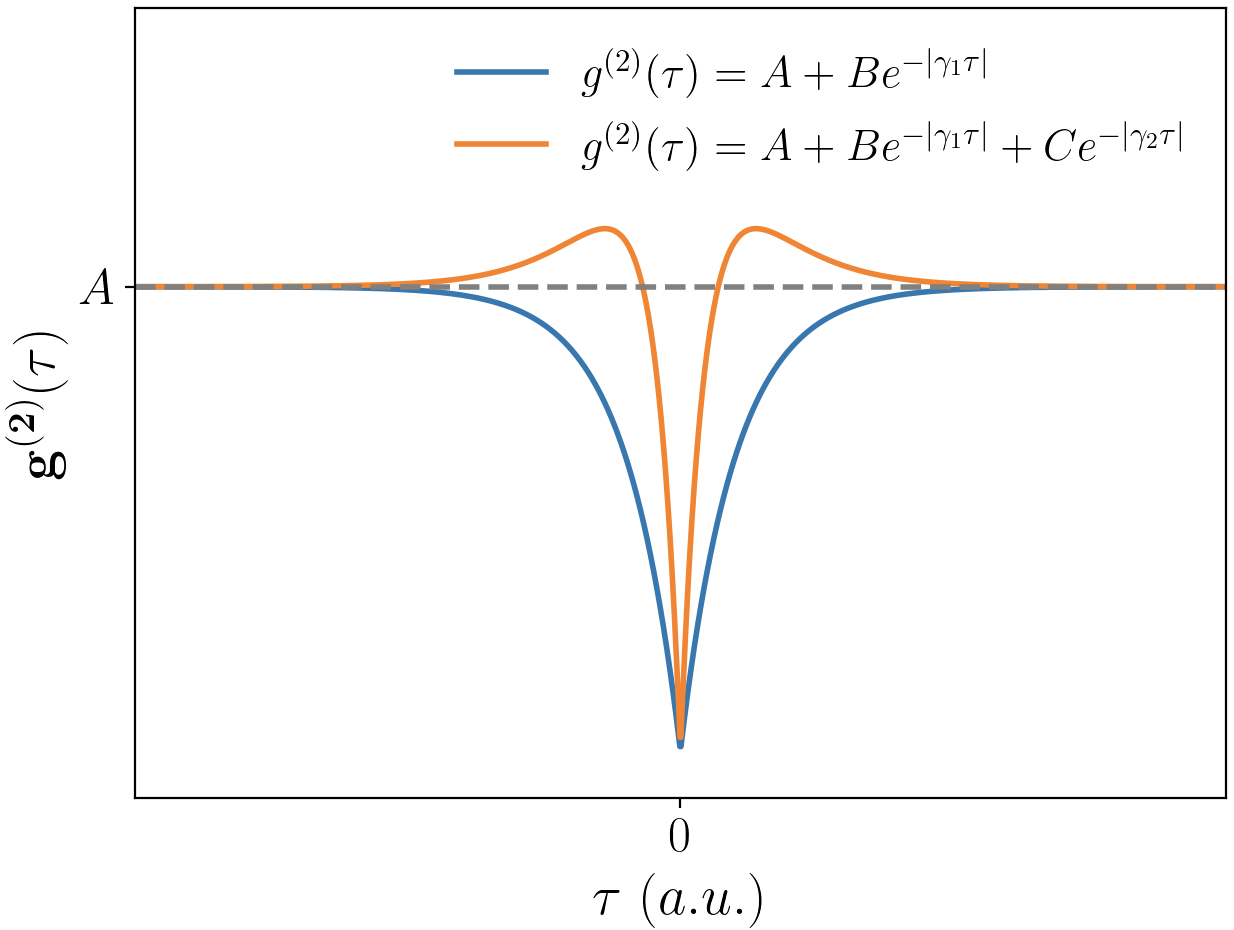
\includegraphics[width=0.7\linewidth]{Figures/g2Visualisation.png}
    \caption{Visualisation of the different $g^{(2)}(\tau)$ fits. The orange line depicts Eqn.~\ref{eqn:bi-decay-g2} and exhibits bunching behaviour. The blue line shows Eqn.~\ref{eqn:single-decay-g2} and exhibits no bunching.}
    \label{fig:g2-visualisation}
\end{figure}

where $A$ is the baseline offset, $B$ and $C$ are the amplitudes of the respective decay components, and $t_0$ and $t_1$ are the associated decay time constants. For an ideal two-level system, a single-exponential model is sufficient to describe the dynamics. However, hBN-based single-photon emitters often exhibit competing recombination pathways that create more complex population dynamics \cite{Boll2020}. In these cases, a bi-exponential model is required to fit the $g^{(2)}(\tau)$ curve accurately and account for additional relaxation channels. The zero-delay value, $g^{(2)}(0)$, is obtained by normalising the coincidence counts at $\tau=0$ to the baseline at large time delays. For the bi-exponential model, this yields $(A + B + C)/A$, while in the single-exponential case it simplifies to $(A + B)/A$.

Under pulsed excitation, the $g^{(2)}(\tau)$ histogram appears as a series of peaks separated by the laser repetition period. To extract $g^{(2)}(0)$, the area under the peak at $\tau=0$ is divided by the mean area of peaks at longer delays. It is essential to measure over sufficiently long time windows to capture any photon bunching effects, which can elevate peaks near zero delay and otherwise distort the calculated $g^{(2)}(0)$ value.


\subsubsection[Michelson Interferometer and Dephasing Rate]{Michelson Interferometer and $\Gamma$}

The Michelson interferometer (see Fig.~\ref{fig:setup}) is used to measure the degree of first-order coherence of a single-photon wavepacket by quantifying its ability to interfere with itself. When the two interferometer arms are equal in length ($\tau=0$, Fig.~\ref{fig:MachZhenderMichelson}), the wavepacket overlaps perfectly in time, producing maximum intensity at one output of the beam splitter and minimum at the other. As the delay $\tau$ is varied, the interference pattern oscillates: for example, a shift of $\tau=\lambda/(2c)$, where $\lambda$ is the wavelength and $c$ the speed of light, introduces a phase shift of $\pi$, swapping constructive and destructive interference between the outputs. By scanning fine delays on the order of a few wavelengths, an interference fringe pattern is observed. The visibility of this pattern is given by:

\begin{equation}
    V = \frac{I_\text{max} - I_\text{min}}{I_\text{max} + I_\text{min}},
    \label{eqn:vis}
\end{equation}

where $I_\text{max}$ and $I_\text{min}$ are the maximum and minimum fringe intensities. Perfect phase coherence at $\tau=0$ yields $V=1$, but the visibility decays exponentially at a rate of $\Gamma/2$ as $\tau$ increases. For emitters with fast dephasing, such as hBN defects at room temperature, this decay is much faster than for emitters at cryogenic temperatures This behaviour can be understood by considering how a pure single-photon state evolves when passing through the Michelson interferometer.

A pure (perfectly indistinguishable) single-photon can be described as \cite{Maffei2021}:

\begin{equation}
\begin{aligned}
    \ket{1} & = -i\int_{-\infty}^{\infty} dt\, \sqrt{\gamma} e^{-\frac{t}{2}(\gamma+2i\omega_0)} \Theta(t) \hat{a}^{\dagger}(t) \ket{0}, \\
    & = \int_{-\infty}^{\infty} dt f(t) \hat{a}^{\dagger}(t) \ket{0},
    \label{eqn:wavepacket}
\end{aligned}
\end{equation}

where $\gamma$ is the spontaneous decay rate of the emitter, $\omega_0$ is the central frequency of the single-photon wavepacket, $\Theta(t)$ is the Heaviside step function (ensuring only positive times are considered), and $\hat{a}^{\dagger}(t)$ is the time-dependent photon creation operator in the Fock basis. 

In the presence of pure dephasing at rate $\gamma^*$, the input photon density matrix is modified as:

\begin{equation}
    \rho_{in} = \int_{-\infty}^{\infty}\int_{-\infty}^{\infty}dt \ dt' f(t)f^*(t') \hat{a}^{\dagger}(t) \ket{0} \bra{0} \hat{a}(t) e^{-\gamma^*|t-t'|}.
\end{equation}

Although real dephasing sources are typically non-Markovian process', meaning that the dephasing rate at a given time depends on all the system's previous states, it can be approximated as a Markovian exponential decay of the form $e^{-\gamma^*|t-t'|}$. This is because the environmental fluctuations and phonon interactions are assumed to act instantaneously in comparison to the timescale of the photon dephasing.

To model the evolution of this state through a Michelson interferometer, it is convenient to consider the topologically equivalent case of a Mach–Zehnder interferometer with one delayed arm, as illustrated in Fig.~\ref{fig:MachZhenderMichelson}. 


\begin{figure}[h]
    \centering
    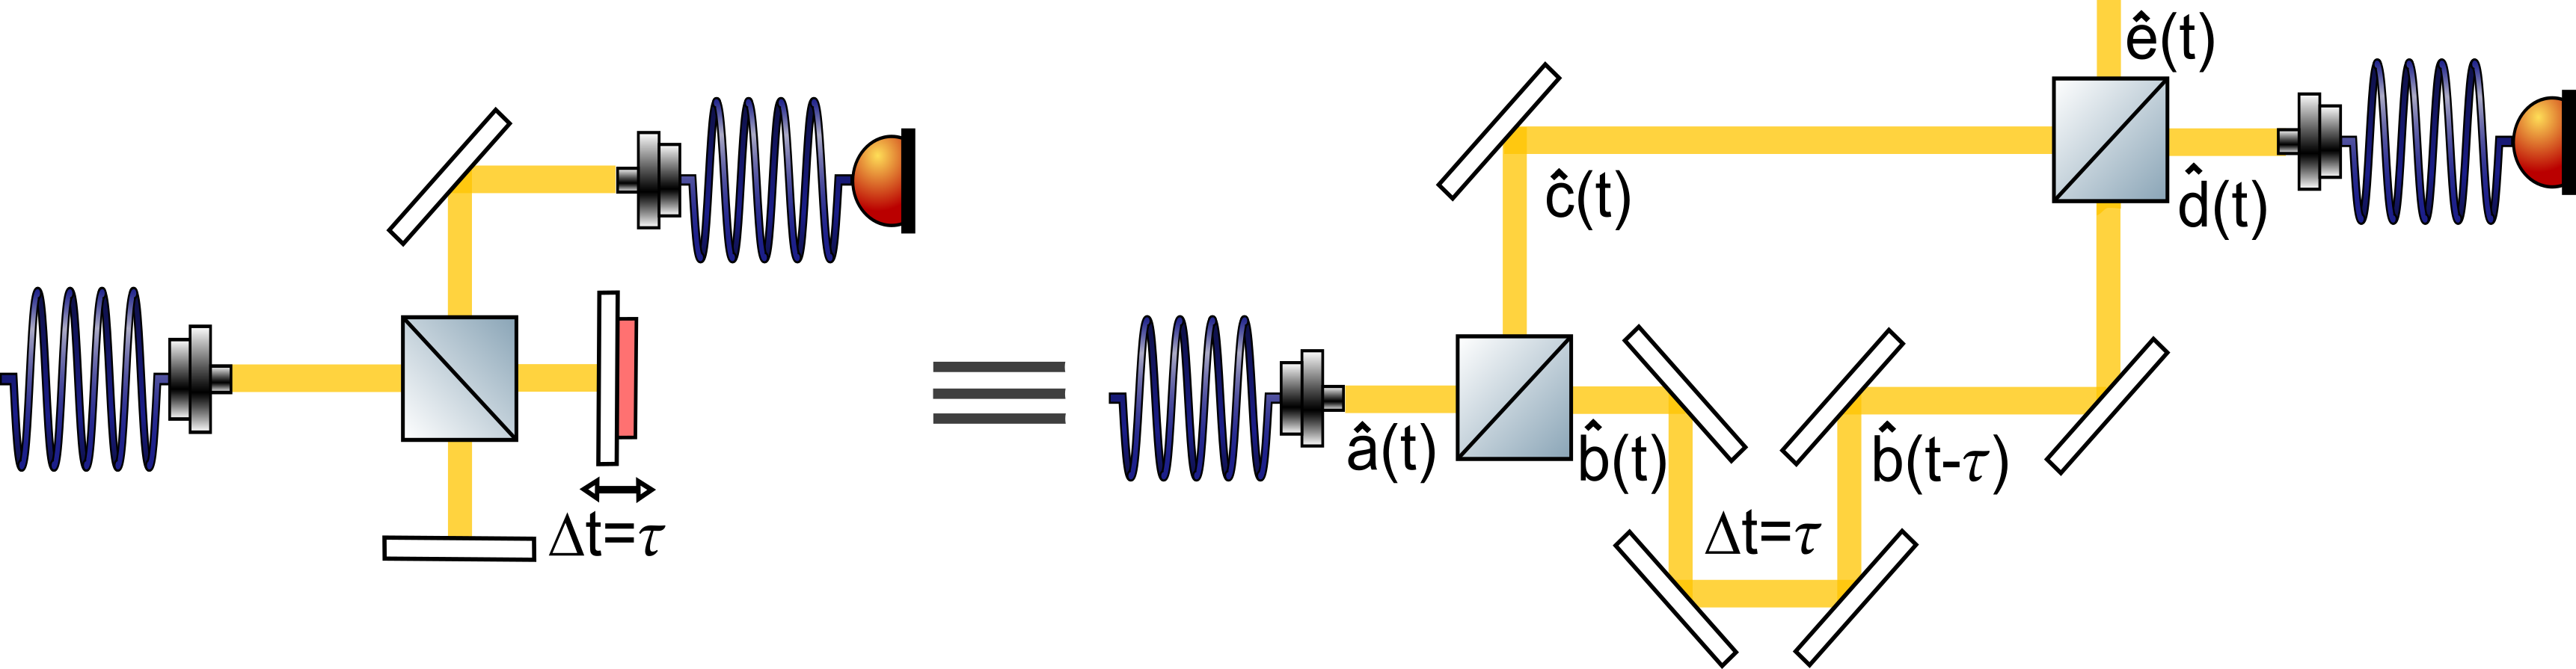
\includegraphics[width=0.8\linewidth]{Figures/MachZhenderMichelson.png}
    \caption{Equivalence of a Mach Zhender interferometer with time delay $\tau$ and a Michelson interferometer. They are both topologically equivalent, and an analysis of the Mach-Zhender is performed for ease.}
    \label{fig:MachZhenderMichelson}
\end{figure}

As the photon passes through a beam splitter, it has a 50:50 probability of being transmitted or reflected. The beam splitter can therefore be described by an operator that splits the field between the two output modes. When the photon passes through a path delay in one arm, the field operator is then shifted in time, acting at a later time by $\tau$. Using standard beam splitter conventions \cite{Gerry2005}, the field operators evolve as:


\begin{align}
    \hat{a}(t) & \rightarrow \frac{1}{\sqrt{2}}\left(\hat{b}(t) + \hat{c}(t) \right) \label{eqn:MZ1}\\
    \hat{b}(t) & \rightarrow \hat{b}(t-\tau) \label{eqn:MZ2}\\
    \hat{b}(t-\tau) & \rightarrow \frac{1}{\sqrt{2}}\left(\hat{e}(t-\tau) + \hat{d}(t-\tau) \right) \label{eqn:MZ3}\\
    \hat{c}(t) & \rightarrow \frac{1}{\sqrt2} \left( \hat{e}(t)-\hat{d}(t)\right) \label{eqn:MZ4}
\end{align}

Applying these transformations, the output density matrix becomes:

\begin{equation}
\begin{aligned}
    \rho_{out} = \int_{-\infty}^{\infty}\int_{-\infty}^{\infty}dt \ dt' f(t)f^*(t') e^{-\gamma^*|t-t'|} \times \\ 
    \left[\hat{d}^{\dagger}(t)+\hat{d}^{\dagger}(t-\tau)-\hat{e}^{\dagger}(t) + \hat{e}^{\dagger}(t-\tau)\right]
    \ket{0} \bra{0} \times \\
    \left[\hat{d}(t)+\hat{d}(t-\tau)-\hat{e}(t) + \hat{e}(t-\tau)\right],
\end{aligned}
\end{equation}

The photon intensity measured at output port $\hat{d}(t)$ is given by:

\begin{equation}
\begin{aligned}
    N_d(t'') 
    &= \langle \hat{d}^{\dagger}(t'') \hat{d}(t'') \rangle 
    = \text{Tr}\left[\hat{\rho}_{out} \, \hat{d}^{\dagger}(t'') \hat{d}(t'')\right] \\
    &= \int_{-\infty}^{\infty} \int_{-\infty}^{\infty} dt \, dt' \, f(t) f e^{-\gamma^*|t - t'|} \\
    &\quad \times \text{Tr} \Big[ 
        \left( \hat{d}^{\dagger}(t) + \hat{d}^{\dagger}(t - \tau) 
              - \hat{e}^{\dagger}(t) + \hat{e}^{\dagger}(t - \tau) \right) 
        \ket{0} \bra{0} \\
    &\hspace{1.7cm}
         \left( \hat{d}(t) + \hat{d}(t - \tau) 
              - \hat{e}(t) + \hat{e}(t - \tau) \right)
        \hat{d}^{\dagger}(t'') \hat{d}(t'') 
    \Big] \\
    &= \int_{-\infty}^{\infty} \int_{-\infty}^{\infty} dt \, dt' \, f(t) f^*(t') e^{-\gamma^*|t - t'|} \\
    &\quad \times \big[ 
        \delta(t - t'') \delta(t' - t'') 
        + \delta(t - \tau - t'') \delta(t' - t'') \\
    &\qquad 
        + \delta(t - t'') \delta(t' - \tau - t'') 
        + \delta(t - \tau - t'') \delta(t' - \tau - t'') 
    \big] \\
    &= |f(t'')|^2 + |f(\tau+t'')|^2 + 2\text{Re}\left[f(t'')f^*(\tau+t'')e^{-\gamma^* \tau } \right]\\
\end{aligned}
\end{equation}

For the wavepacket described in equation~\ref{eqn:wavepacket}, this results in:

\begin{equation}
    N_d(t'') = \frac{\gamma}{4} e^{-\gamma t''} \left[\Theta(t'') + \Theta(t'' - \tau) e^{-\gamma \tau} + 2 \cos(\omega_0 \tau)\, e^{-\gamma t'' - \gamma^* \tau} \Theta(t'') \Theta(t'' - \tau) \right].
\end{equation}

Integrating over all time gives the total photon number at detector $\hat{d}$:

\begin{equation}
\begin{aligned}
    N_d &= \int_{-\infty}^{\infty} dt''\, N_d(t'') \\
        &= \frac{1}{2} \left(1 + e^{-\frac{1}{2}(\gamma + 2\gamma^*) \tau} \cos(\omega_0 \tau) \right) \\
        &= \frac{1}{2} \left(1 + e^{-\frac{1}{2} \Gamma \tau} \cos(\omega_0 \tau) \right),
        \label{eqn:int-decay}
\end{aligned}
\end{equation}

\begin{figure}[h!]
    \centering
    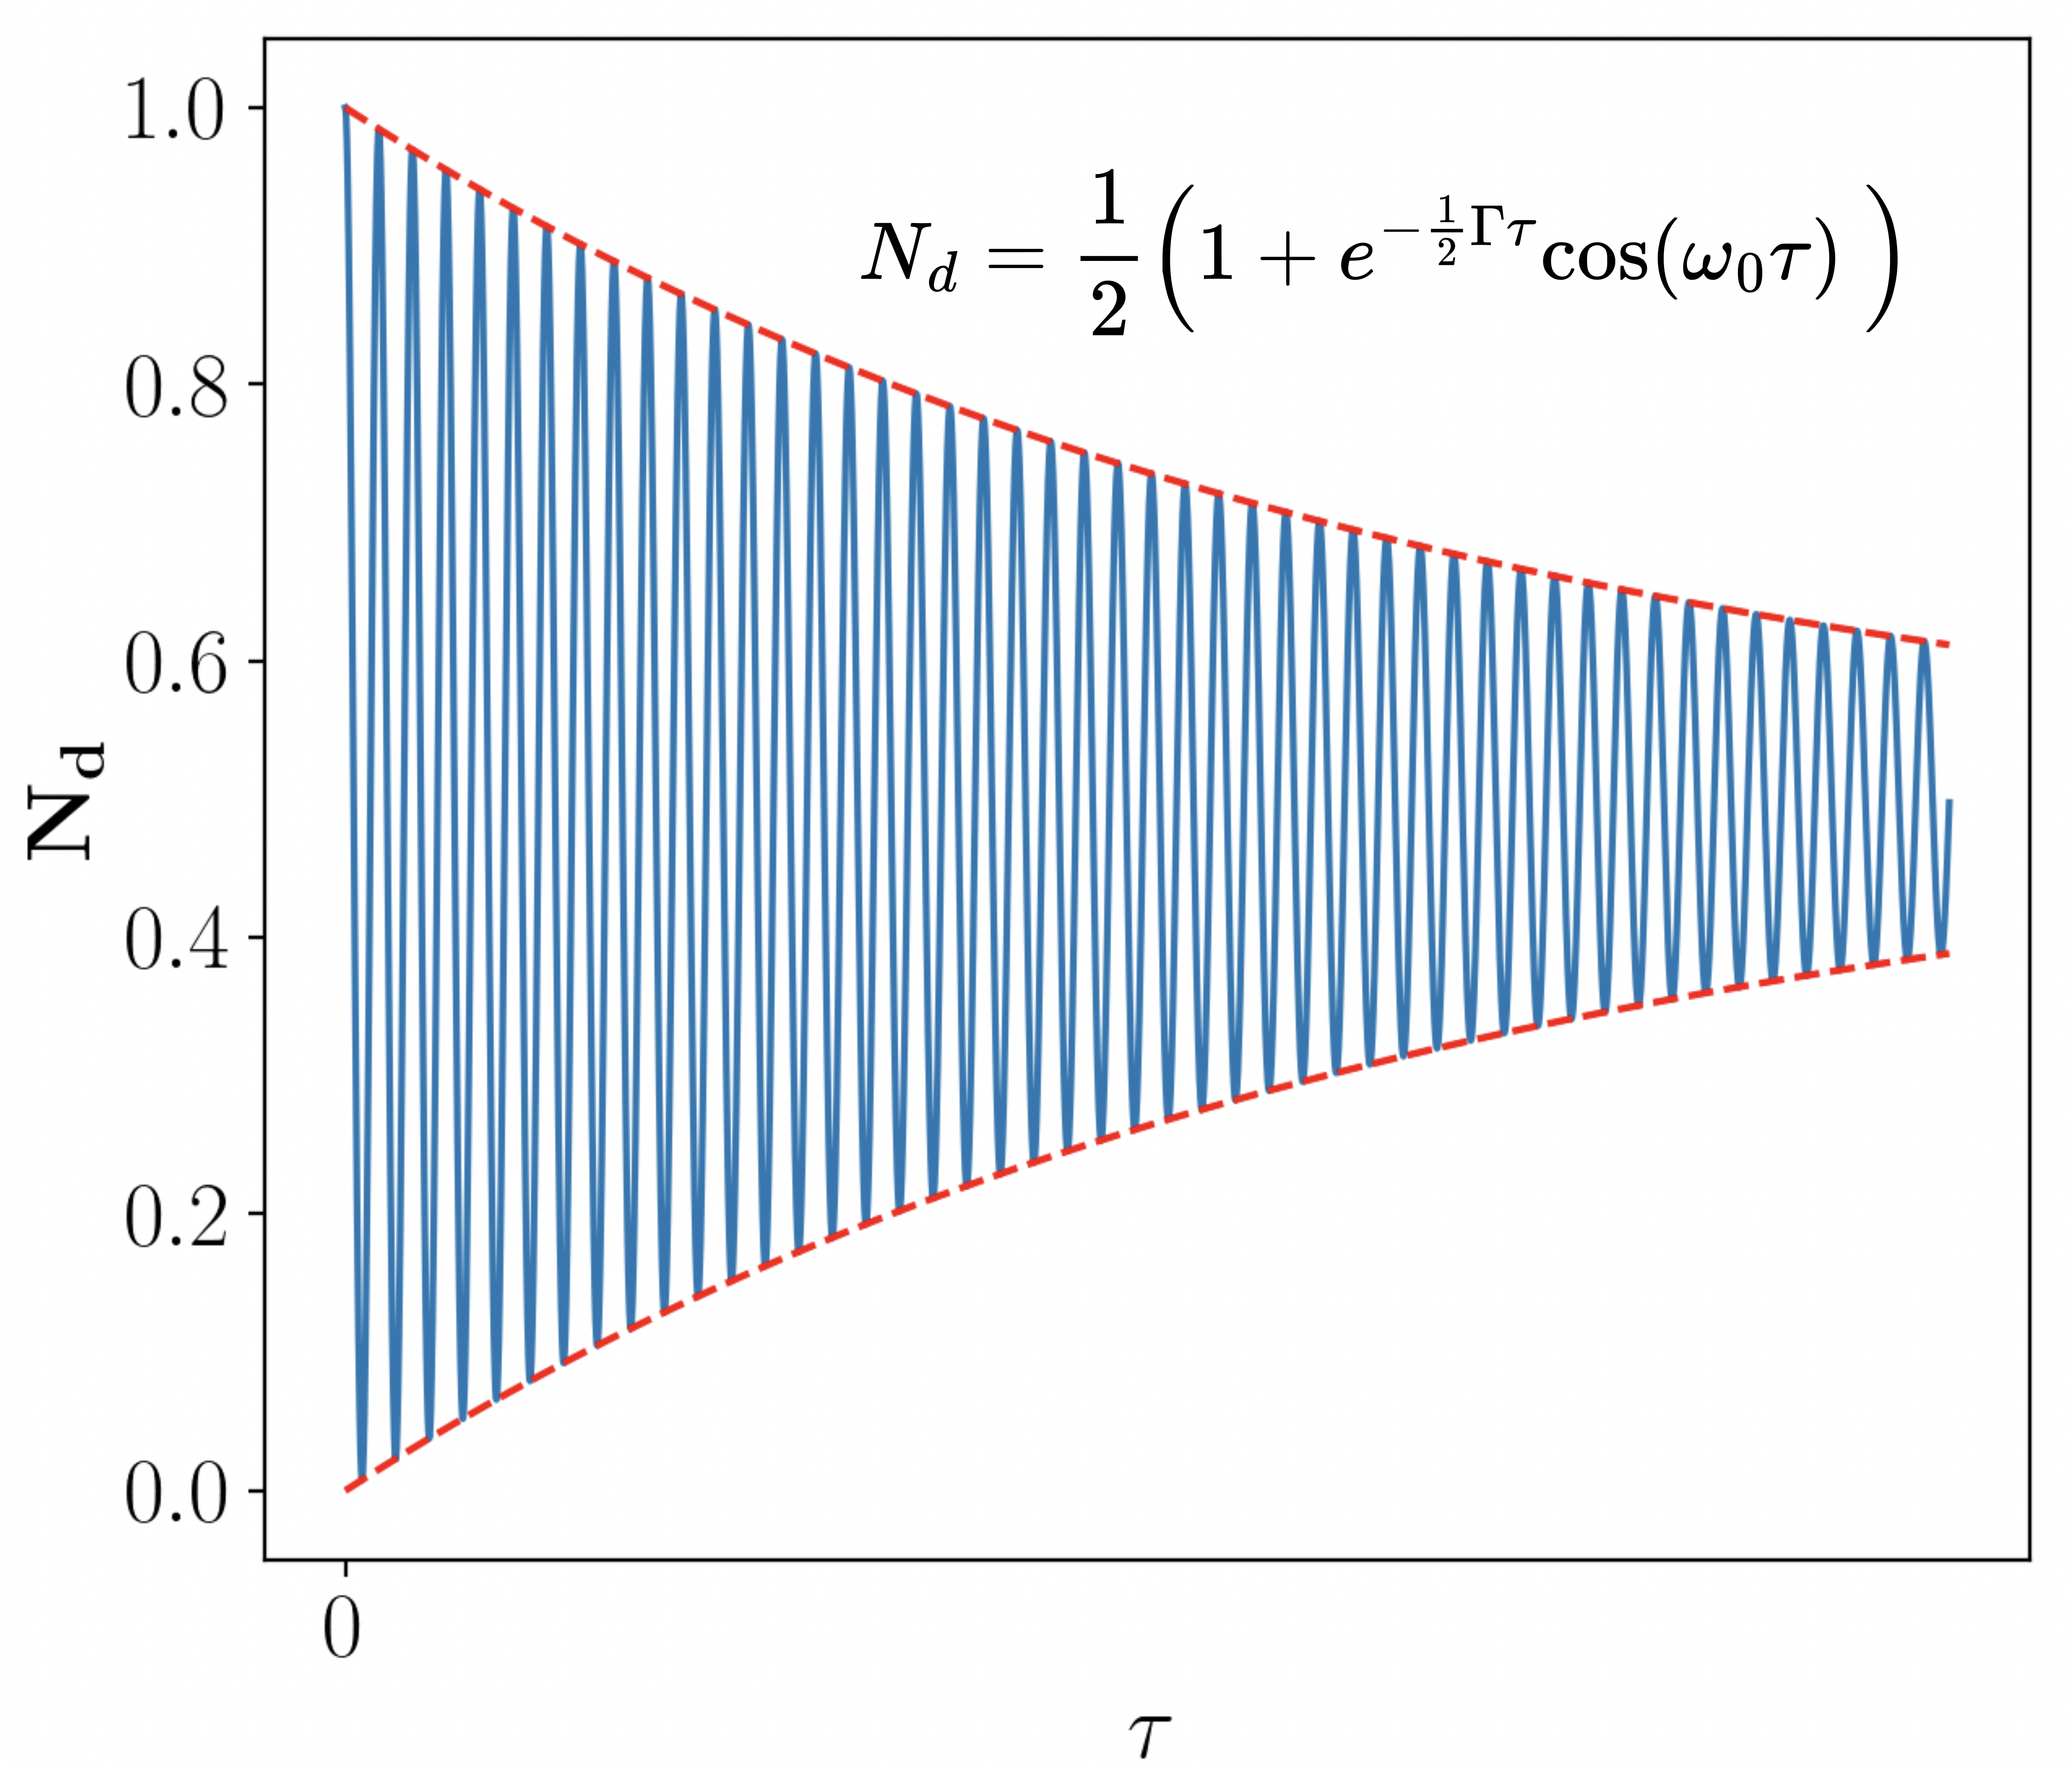
\includegraphics[width=0.8\linewidth]{Figures/VisDecay.png}
    \caption{Graphical representation of decay in intensity  $N_d(t)$ as a function of delay, $\tau$}
    \label{fig:visdecay}
\end{figure}


This result shows that the measured intensity at the output oscillates with frequency $\omega_0$ and decays exponentially with delay $\tau$ due to the combined effect of spontaneous emission and pure dephasing, Fig.~\ref{fig:visdecay}. Using Eqn.~\ref{eqn:vis} and ~\ref{eqn:int-decay}, it can be shown that the visibility decays with path delay as:

\begin{equation}
    V(\tau)=e^{-\frac{\Gamma}{2}\tau}.
    \label{eqn:vis-decay}
\end{equation}

The envelope of this decay allows a direct measurement of the emitter's coherence properties and extraction of the total dephasing rate $\Gamma$.

The piezo holding the mirror has a range of 20~$\mu$m, corresponding to a path delay of approximately $30\lambda$ or 70~fs, while the translation stage used for coarse adjustment provides up to 5~mm displacement, equivalent to several thousand wavelengths or about 10~ps. During measurements, the piezo is driven by a 10~Hz triangular waveform varying between 0.5~V and 9.5~V, producing an 18~$\mu$m peak-to-peak displacement without reaching the piezo’s limit. The interferometer output is coupled into single-mode fibre and sent to an APD. A synchronised square wave at the same frequency triggers the QuTag TCSPC, ensuring that the measured delay resets to zero each cycle so the intensity at each point corresponds accurately to the piezo position. The visibility of the interference pattern is calculated at each position of the translation stage, and the measurement is repeated across the full range to capture the decay of visibility over long time delays. All raw time-tagged data are analysed with the \textit{Extensible Time-tag Analyzer} (\textit{ETA}) \cite{Lin2021}, enabling custom histogram generation with adjustable bin sizes for flexible analysis over short and long timescales.



